
\chapter{The Geo-Cloud Experiment}

The GEO-Cloud experiment consists of the emulation of a realistic and complete Earth Observation System that provides services using cloud technology. For that purpose a constellation of satellites, ground stations, a cloud architecture, use cases and end users' models are designed.

The \acs{EO} system will be computed and emulated in \emph{Fed4FIRE}: A constellation of satellites record images of the Earth in a daily basis. The images are transferred to ground stations that ingest the data into a cloud computing infrastructure. The data is processed and distributed to end users.

The GEO-Cloud experiment is tested in three testbeds: \vw,\bonfire and
\pl. GEO-Cloud is divided into two sub-experiments:
\begin{itemize}
\item One experiment in a system integrated in \vw and \bonfire.
\item One experiment in \pl.
\end{itemize}

The experiment in \vw and \bonfire emulates the whole \acs{EO} system. In \vw:
constellation of satellites, the ground stations and the end users' models. In
\bonfire the cloud architecture, the processing chain of the data and its
distribution. Both \vw and \bonfire are interconnected to transfer information from one testbed to the other and viceversa.

The experiment in \pl consists of the emulation of the networks that constitute
the links between the ground stations to the cloud and from the cloud to the end
users. There, the network performance, features, bandwidth and impairments are
monitored and measured. Those parameters once measured are used to update the
models implemented in \vw, i.e, bandwidth, latency and loss rate.

In the next sections, the detailed design of the GEO-Cloud experiment is introduced.

\section{Satellite System Design}
\label{subsec:system-design}
\subsection{Design of the flight and ground segments}
\label{subsubsec:design-flight-ground}
In this subsection, the main characteristics of the system are presented. Objectives, constraints, previous estimations and possible modifications and their effects in the system are exposed.

In a wide vision, it is an \acs{EO} system consisting of a constellation of satellites equally spaced in a \acs{LEO} orbit with the aim of achieving daily coverage of the entire Earth surface. These conditions imply a very sophisticated handle of a huge quantity of data.

The following requirements have been fulfilled to design the system:
\begin{itemize}
\item Swath: $160km$ (based on state of the art cameras).
\item Resolution: $6.7m$ (based on state of the art cameras).
\item Low Earth Orbits.
\item Sun Synchronous orbits.
\item Download data rate: $160 Mbps$ (based on Deimos-2 satellite characteristics).
\item Optical Bands: 5 Multispectral (based on state of the art cameras).
\end{itemize}

\paragraph{Global Daily Coverage}~\\
The objective of this system is the acquisition of images of the total Earth surface in a daily basis. Global coverage is considered to include the land surface that is shown in Figure~\ref{fig:intr-land-surface}.


\begin{figure}[!h]
\begin{center}
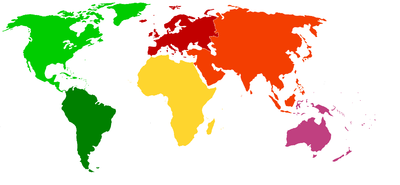
\includegraphics[width=0.6\textwidth]{detaildesign/surface-daily.png}
\caption{Land surface to be acquired in a daily basis}
\label{fig:intr-land-surface}
\end{center}
\end{figure}


\paragraph{Flight Segment}~\\
The satellites are selected according to the current state of the art. However,
some enhancements can be assumed as a way to adjust the analysis to the short
term future.


\subparagraph{Satellite performances}~\\
As a first iteration for the system, small platforms of less of $500kg$ are supposed according to the size and payload bay characteristics of representative platforms in this category. This study is based on the bus platforms currently offered by Surrey Satellite Technology Ltd, Satrec Initiative, Sierra Nevada Corporation, etcetera.

To reduce the amount of satellites orbiting the Earth, a design with two payloads has been assumed. Thus, the swath (the width of the field of view of each satellite in the surface of the Earth) can be duplicated without decreasing the resolution.

The satellites shall be pointing to nadir, acquiring images without maneuvering because of the acquisition plan for cover the Earth daily. Simultaneously, when a satellite gets into the field of view of a Ground Station, the download starts and at the same time the satellite continues imaging.

The main specifications of the satellites in the constellation are shown in Table~\ref{table:intro-satellite-performances}. The values of each parameter have been selected according to the state of the art and the desired quality of the images in the mission.

\begin{table}[hp]
  \centering
  {\small
  


\begin{tabular}{p{.2\textwidth}p{.2\textwidth}}
  \tabheadformat
  \tabhead{Specification}   &
  \tabhead{Value}\\
\hline
\textit{GSD}         & $6.7~m$ \\
\hline
\textit{Swath}         & $160~km$ \\
\hline
\textit{Number of bands}         & $5$ \\
\hline
\textit{Digitalization}         & $12~bits$ \\
\hline
\textit{Download Data Rate}         & $160~Mbps$ \\
\hline
\textit{Compression Rate}         &  $2:1$\\
\hline

\end{tabular}


% Local variables:
%   coding: utf-8
%   ispell-local-dictionary: "castellano8"
%   TeX-master: "main.tex"
% End:

  }
  \caption{Main Performances of the Satellites}
  \label{table:intro-satellite-performances}
\end{table}


\subparagraph{Orbit definition}~\\
It is common in \acs{EO} satellite missions the use of \emph{sun-synchronous} orbits. These orbits guarantee that the lighting conditions of the imaged places are the same during the mission, which is a very desirable characteristic.

\acs{LTAN} is also a desired condition of the orbit very related to the lighting and weather conditions of those places that the satellite overflies (\acs{LTAN} is selected according to the desired local time of the overflown places and the cloud formation during the day); it is common the use of \emph{LTAN 10:30h} for Earth Observation.

Other of the main parameters of an orbit is the altitude. Altitude has effects in the resolution and the swath of the satellites, which has impact in the number of satellites required to achieve the coverage objective. According to the value of those parameters in the payloads included in the satellites, the reference altitude for the system was found to be \emph{646km}. \acs{SSO} condition implies a relation between the altitude and the inclination of the orbit of \emph{97.97deg} in this case.

\subparagraph{Number of satellites in the constellation}~\\
The number of satellites shall be calculated using the altitude ($646 km$), the
inclination ($97.97 deg$) and a swath in
Table~\ref{table:intro-satellite-performances}. As a result, 17 satellites are
required to carry out this mission. In Figure~\ref{fig:intr-constellation-global} the whole constellation is
shown.

\begin{figure}[!h]
\begin{center}
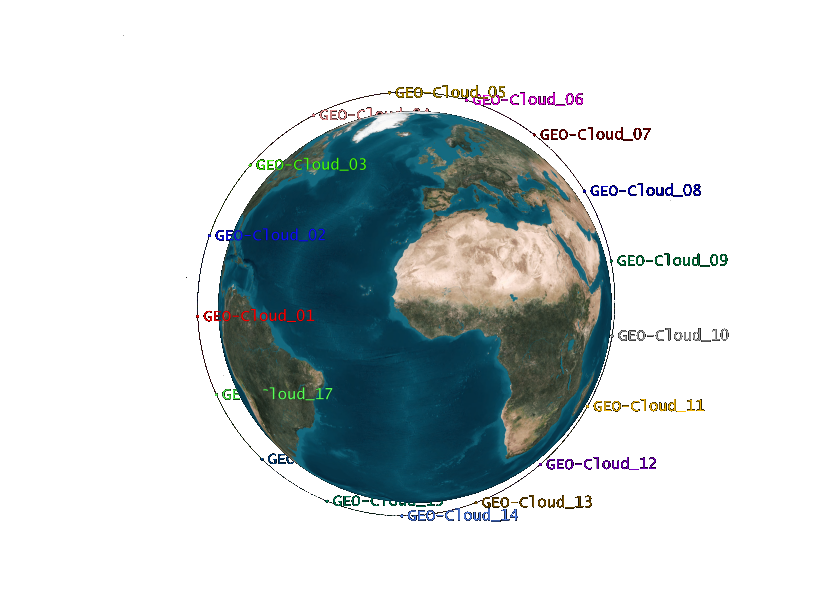
\includegraphics[width=0.6\textwidth]{detaildesign/constellation-global.png}
\caption{Constellation of 17 satellites in a SSO orbit at 646km}
\label{fig:intr-constellation-global}
\end{center}
\end{figure}

\paragraph{Ground Stations design}~\\
When the satellite acquires the data, it has to be downloaded to the Ground
Stations and then it has to be distributed to the customers. Due to the huge
quantity of data and the limitations the download data rate sets, several
stations distributed over the surface of the Earth are required. They will allow
the satellite to communicate with them and download the images. Due the
accumulated duration of the accesses to all the ground stations per day and the
frequency of accesses per day (it varies with the latitude of the station), the
Figure~\ref{fig:intr-footprints} shows how the Ground Stations and its
footprints (area in which the satellites can communicate with the Ground
Station) is distributed.


\begin{figure}[!h]
\begin{center}
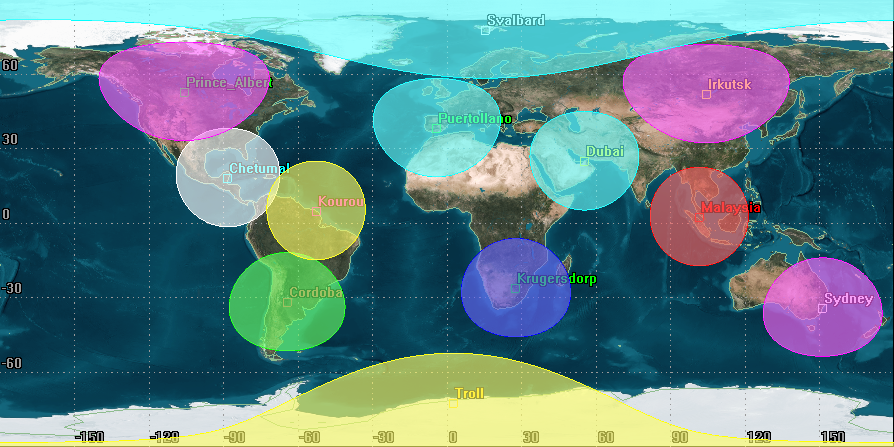
\includegraphics[width=0.8\textwidth]{detaildesign/footprints.png}
\caption{Footprints of the selected Ground Stations}
\label{fig:intr-footprints}
\end{center}
\end{figure}

\subsection{Generated Data Volume}

Specifically, $135,698,500 km^2$ of ground surface are daily acquired. With the following expression can estimate the data volume generated:

\begin{equation}
Acquired~Data~Volume= \frac{Acquired~Surface}{GSD^2} * Nº bands * Digitalization
\end{equation}

Before downloading the images they are compressed. The ancillary data is
included in the process (auxiliary information useful for the geolocation of the
images, protocol \ldots). In this case, the ancillary data is estimated to be
12\% of the acquired data (based on Deimos 2 satellite measurements), which is
added and then compressed. With the values depicted in
Table~\ref{table:intro-satellite-performances}, the ancillary and the daily ground
surface adquired, the data on ground can be estimated. As result including ancillary data before compression, \emph{11.55TBytes} shall be downloaded daily.

